%  A simple AAU report template.
%  2015-05-08 v. 1.2.0
%  Copyright 2010-2015 by Jesper Kjær Nielsen <jkn@es.aau.dk>
%
%  This is free software: you can redistribute it and/or modify
%  it under the terms of the GNU General Public License as published by
%  the Free Software Foundation, either version 3 of the License, or
%  (at your option) any later version.
%
%  This is distributed in the hope that it will be useful,
%  but WITHOUT ANY WARRANTY; without even the implied warranty of
%  MERCHANTABILITY or FITNESS FOR A PARTICULAR PURPOSE.  See the
%  GNU General Public License for more details.
%
%  You can find the GNU General Public License at <http://www.gnu.org/licenses/>.
%
%  A simple AAU report template.
%  2015-05-08 v. 1.2.0
%  Copyright 2010-2015 by Jesper Kjær Nielsen <jkn@es.aau.dk>
%
%  This is free software: you can redistribute it and/or modify
%  it under the terms of the GNU General Public License as published by
%  the Free Software Foundation, either version 3 of the License, or
%  (at your option) any later version.
%
%  This is distributed in the hope that it will be useful,
%  but WITHOUT ANY WARRANTY; without even the implied warranty of
%  MERCHANTABILITY or FITNESS FOR A PARTICULAR PURPOSE.  See the
%  GNU General Public License for more details.
%
%  You can find the GNU General Public License at <http://www.gnu.org/licenses/>.
%
\documentclass[11pt,twoside,a4paper,openany]{report}
%%%%%%%%%%%%%%%%%%%%%%%%%%%%%%%%%%%%%%%%%%%%%%%%
% Language, Encoding and Fonts
% http://en.wikibooks.org/wiki/LaTeX/Internationalization
%%%%%%%%%%%%%%%%%%%%%%%%%%%%%%%%%%%%%%%%%%%%%%%%
% Select encoding of your inputs. Depends on
% your operating system and its default input
% encoding. Typically, you should use
%   Linux  : utf8 (most modern Linux distributions)
%            latin1 
%   Windows: ansinew
%            latin1 (works in most cases)
%   Mac    : applemac
% Notice that you can manually change the input
% encoding of your files by selecting "save as"
% an select the desired input encoding. 
\usepackage[utf8]{inputenc}
% Make latex understand and use the typographic
% rules of the language used in the document.
\usepackage[danish]{babel}

% Use the palatino font
\usepackage[sc]{mathpazo}
\linespread{1.05}         % Palatino needs more leading (space between lines)
% Choose the font encoding
\usepackage[T1]{fontenc}
%%%%%%%%%%%%%%%%%%%%%%%%%%%%%%%%%%%%%%%%%%%%%%%%
% Graphics and Tables
% http://en.wikibooks.org/wiki/LaTeX/Importing_Graphics
% http://en.wikibooks.org/wiki/LaTeX/Tables
% http://en.wikibooks.org/wiki/LaTeX/Colors
%%%%%%%%%%%%%%%%%%%%%%%%%%%%%%%%%%%%%%%%%%%%%%%%
% load a colour package
\usepackage{xcolor}
\definecolor{aaublue}{RGB}{33,26,82}% dark blue
% The standard graphics inclusion package
\usepackage{graphicx}
% Set up how figure and table captions are displayed
\usepackage{caption}
\captionsetup{%
  font=footnotesize,% set font size to footnotesize
  labelfont=bf % bold label (e.g., Figure 3.2) font
}
% Make the standard latex tables look so much better
\usepackage{array,booktabs}
% Enable the use of frames around, e.g., theorems
% The framed package is used in the example environment
\usepackage{framed}

%%%%%%%%%%%%%%%%%%%%%%%%%%%%%%%%%%%%%%%%%%%%%%%%
% Mathematics
% http://en.wikibooks.org/wiki/LaTeX/Mathematics
%%%%%%%%%%%%%%%%%%%%%%%%%%%%%%%%%%%%%%%%%%%%%%%%
% Defines new environments such as equation,
% align and split 
\usepackage{amsmath}
% Adds new math symbols
\usepackage{amssymb}
% Use theorems in your document
% The ntheorem package is also used for the example environment
% When using thmmarks, amsmath must be an option as well. Otherwise \eqref doesn't work anymore.
\usepackage[framed,amsmath,thmmarks]{ntheorem}

%%%%%%%%%%%%%%%%%%%%%%%%%%%%%%%%%%%%%%%%%%%%%%%%
% Page Layout
% http://en.wikibooks.org/wiki/LaTeX/Page_Layout
%%%%%%%%%%%%%%%%%%%%%%%%%%%%%%%%%%%%%%%%%%%%%%%%
% Change margins, papersize, etc of the document
\usepackage[
  inner=28mm,% left margin on an odd page
  outer=41mm,% right margin on an odd page
  ]{geometry}
% Modify how \chapter, \section, etc. look
% The titlesec package is very configureable
\usepackage{titlesec}
\titleformat{\chapter}[display]{\normalfont\huge\bfseries}{\chaptertitlename\ \thechapter}{20pt}{\Huge}
\titleformat*{\section}{\normalfont\Large\bfseries}
\titleformat*{\subsection}{\normalfont\large\bfseries}
\titleformat*{\subsubsection}{\normalfont\normalsize\bfseries}
%\titleformat*{\paragraph}{\normalfont\normalsize\bfseries}
%\titleformat*{\subparagraph}{\normalfont\normalsize\bfseries}

% Change the headers and footers
\usepackage{fancyhdr}
\pagestyle{fancy}
\fancyhf{} %delete everything
\renewcommand{\headrulewidth}{0pt} %remove the horizontal line in the header
\fancyhead[RE]{\small\nouppercase\leftmark} %even page - chapter title
\fancyhead[LO]{\small\nouppercase\rightmark} %uneven page - section title
\fancyhead[LE,RO]{\thepage} %page number on all pages
% Do not stretch the content of a page. Instead,
% insert white space at the bottom of the page
\raggedbottom
% Enable arithmetics with length. Useful when
% typesetting the layout.
\usepackage{calc}

%%%%%%%%%%%%%%%%%%%%%%%%%%%%%%%%%%%%%%%%%%%%%%%%
% Bibliography
% http://en.wikibooks.org/wiki/LaTeX/Bibliography_Management
%%%%%%%%%%%%%%%%%%%%%%%%%%%%%%%%%%%%%%%%%%%%%%%%
\usepackage[backend=biber,
  bibencoding=utf8,
  style=apa,
  %citestyle=apa,
  language=danish
  ]{biblatex}
\bibliography{bib/mybib}
\DeclareLanguageMapping{danish}{danish-apa}
\DefineBibliographyStrings{danish}{
    bibliography = {Kildeliste},
    references = {Kildeliste}
    }
%%%%%%%%%%%%%%%%%%%%%%%%%%%%%%%%%%%%%%%%%%%%%%%%
% Misc
%%%%%%%%%%%%%%%%%%%%%%%%%%%%%%%%%%%%%%%%%%%%%%%%
% Add bibliography and index to the table of
% contents
\usepackage[nottoc]{tocbibind}
% Add the command \pageref{LastPage} which refers to the
% page number of the last page
\usepackage{lastpage}
% Add todo notes in the margin of the document
\usepackage[
%  disable, %turn off todonotes
  colorinlistoftodos, %enable a coloured square in the list of todos
  textwidth=\marginparwidth, %set the width of the todonotes
  textsize=scriptsize, %size of the text in the todonotes
  ]{todonotes}

%%%%%%%%%%%%%%%%%%%%%%%%%%%%%%%%%%%%%%%%%%%%%%%%
% Hyperlinks
% http://en.wikibooks.org/wiki/LaTeX/Hyperlinks
%%%%%%%%%%%%%%%%%%%%%%%%%%%%%%%%%%%%%%%%%%%%%%%%
% Enable hyperlinks and insert info into the pdf
% file. Hypperref should be loaded as one of the 
% last packages
\usepackage{hyperref}
\hypersetup{%
	pdfpagelabels=true,%
	plainpages=false,%
	pdfauthor={Author(s)},%
	pdftitle={Title},%
	pdfsubject={Subject},%
	bookmarksnumbered=true,%
	colorlinks=false,%
	citecolor=black,%
	filecolor=black,%
	linkcolor=black,% you should probably change this to black before printing
	urlcolor=black,%
	pdfstartview=FitH%
}
% package inclusion and set up of the document
% see, e.g., http://en.wikibooks.org/wiki/LaTeX/Formatting#Hyphenation
% for more information on word hyphenation
\hyphenation{ex-am-ple hy-phen-a-tion short}
\hyphenation{long la-tex}
% 
%  A simple AAU report template.
%  2015-05-08 v. 1.2.0
%  Copyright 2010-2015 by Jesper Kjær Nielsen <jkn@es.aau.dk>
%
%  This is free software: you can redistribute it and/or modify
%  it under the terms of the GNU General Public License as published by
%  the Free Software Foundation, either version 3 of the License, or
%  (at your option) any later version.
%
%  This is distributed in the hope that it will be useful,
%  but WITHOUT ANY WARRANTY; without even the implied warranty of
%  MERCHANTABILITY or FITNESS FOR A PARTICULAR PURPOSE.  See the
%  GNU General Public License for more details.
%
%  You can find the GNU General Public License at <http://www.gnu.org/licenses/>.
%
%
%
% see, e.g., http://en.wikibooks.org/wiki/LaTeX/Customizing_LaTeX#New_commands
% for more information on how to create macros

%%%%%%%%%%%%%%%%%%%%%%%%%%%%%%%%%%%%%%%%%%%%%%%%
% Macros for the titlepage
%%%%%%%%%%%%%%%%%%%%%%%%%%%%%%%%%%%%%%%%%%%%%%%%
%Creates the aau titlepage
\newcommand{\aautitlepage}[3]{%
  {
    %set up various length
    \ifx\titlepageleftcolumnwidth\undefined
      \newlength{\titlepageleftcolumnwidth}
      \newlength{\titlepagerightcolumnwidth}
    \fi
    \setlength{\titlepageleftcolumnwidth}{0.5\textwidth-\tabcolsep}
    \setlength{\titlepagerightcolumnwidth}{\textwidth-2\tabcolsep-\titlepageleftcolumnwidth}
    %create title page
    \thispagestyle{empty}
    \noindent%
    \begin{tabular}{@{}ll@{}}
      \parbox{\titlepageleftcolumnwidth}{
        \iflanguage{danish}{%
          
\includegraphics[width=\titlepageleftcolumnwidth]{figures/aau_logo_da}
        }{%
          
\includegraphics[width=\titlepageleftcolumnwidth]{figures/aau_logo_en}
        }
      } &
      \parbox{\titlepagerightcolumnwidth}{\raggedleft\sf\small
        #2
      }\bigskip\\
       #1 &
      \parbox[t]{\titlepagerightcolumnwidth}{%
      \textbf{Abstract:}\bigskip\par
        \fbox{\parbox{\titlepagerightcolumnwidth-2\fboxsep-2\fboxrule}{%
          #3
        }}
      }\\
    \end{tabular}
    \vfill
    \iflanguage{danish}{%
      \noindent{\footnotesize\emph{Rapportens indhold er frit tilgængeligt, men offentliggørelse (med kildeangivelse) må kun ske efter aftale med forfatterne.}}
    }{%
      \noindent{\footnotesize\emph{The content of this report is freely available, but publication (with reference) may only be pursued due to agreement with the author.}}
    }
    \clearpage
  }
}

%Create english project info
\newcommand{\englishprojectinfo}[8]{%
  \parbox[t]{\titlepageleftcolumnwidth}{
    \textbf{Title:}\\ #1\bigskip\par
    \textbf{Theme:}\\ #2\bigskip\par
    \textbf{Project Period:}\\ #3\bigskip\par
    \textbf{Project Group:}\\ #4\bigskip\par
    \textbf{Participant(s):}\\ #5\bigskip\par
    \textbf{Supervisor(s):}\\ #6\bigskip\par
    \textbf{Copies:} #7\bigskip\par
    \textbf{Page Numbers:} \pageref{LastPage}\bigskip\par
    \textbf{Date of Completion:}\\ #8
  }
}

%Create danish project info
\newcommand{\danishprojectinfo}[8]{%
  \parbox[t]{\titlepageleftcolumnwidth}{
    \textbf{Titel:}\\ #1\bigskip\par
    \textbf{Tema:}\\ #2\bigskip\par
    \textbf{Projektperiode:}\\ #3\bigskip\par
    \textbf{Projektgruppe:}\\ #4\bigskip\par
    \textbf{Deltager(e):}\\ #5\bigskip\par
    \textbf{Vejleder(e):}\\ #6\bigskip\par
    \textbf{Oplagstal:} #7\bigskip\par
    \textbf{Sidetal:} \pageref{LastPage}\bigskip\par
    \textbf{Afleveringsdato:}\\ #8
  }
}

%%%%%%%%%%%%%%%%%%%%%%%%%%%%%%%%%%%%%%%%%%%%%%%%
% An example environment
%%%%%%%%%%%%%%%%%%%%%%%%%%%%%%%%%%%%%%%%%%%%%%%%
\theoremheaderfont{\normalfont\bfseries}
\theorembodyfont{\normalfont}
\theoremstyle{break}
\def\theoremframecommand{{\color{gray!50}\vrule width 5pt \hspace{5pt}}}
\newshadedtheorem{exa}{Example}[chapter]
\newenvironment{example}[1]{%
		\begin{exa}[#1]
}{%
		\end{exa}
}
% my new macros

\begin{document}
    %frontmatter
    \pagestyle{empty} %disable headers and footers
    \pagenumbering{arabic} %use roman page numbering in the frontmatter
    %  A simple AAU report template.
%  2015-05-08 v. 1.2.0
%  Copyright 2010-2015 by Jesper Kjær Nielsen <jkn@es.aau.dk>
%
%  This is free software: you can redistribute it and/or modify
%  it under the terms of the GNU General Public License as published by
%  the Free Software Foundation, either version 3 of the License, or
%  (at your option) any later version.
%
%  This is distributed in the hope that it will be useful,
%  but WITHOUT ANY WARRANTY; without even the implied warranty of
%  MERCHANTABILITY or FITNESS FOR A PARTICULAR PURPOSE.  See the
%  GNU General Public License for more details.
%
%  You can find the GNU General Public License at <http://www.gnu.org/licenses/>.
%
\pdfbookmark[0]{Front page}{label:frontpage}%
\begin{titlepage}
  \addtolength{\hoffset}{0.5\evensidemargin-0.5\oddsidemargin} %set equal margins on the frontpage - remove this line if you want default margins
  \noindent%
  \begin{tabular}{@{}p{\textwidth}@{}}
    \toprule[2pt]
    \midrule
    \vspace{0.2cm}
    \begin{center}
    \Huge{\textbf{
      P0 projekt% insert your title here
    }}
    \end{center}
    \begin{center}
      \Large{
        - Internet of Things -% insert your subtitle here
      }
    \end{center}
    \vspace{0.2cm}\\
    \midrule
    \toprule[2pt]
  \end{tabular}
  \vspace{4 cm}
  \begin{center}
    {\large
      Project Report%Insert document type (e.g., Project Report)
    }\\
    \vspace{0.2cm}
    {\Large
      A307A%Insert your group name or real names here
    }
  \end{center}
  \vfill
  \begin{center}
  Aalborg University\\
  Datalogi og Software
  \end{center}
\end{titlepage}
\clearpage

    \thispagestyle{empty}
{\small
\strut\vfill % push the content to the bottom of the page
\noindent Copyright \copyright{} Aalborg University 2015\par
\vspace{0.2cm}
\noindent Here you can write something about which tools and software you have used for typesetting the document, running simulations and creating figures. If you do not know what to write, either leave this page blank or have a look at the colophon in some of your books.
}
\newpage


    \selectlanguage{danish}
\pdfbookmark[0]{Danish title page}{label:titlepage_da}
\aautitlepage{%
  \danishprojectinfo{
    P0 projekt - Internet of Things %title
  }{%
    P0 Hvis programmer er løsningen - hvad er så problemet?%theme
  }{%
    Efterårssemestret 2018 %project period
  }{%
    A307a % project group
  }{%
    %list of group members
    Alexander Nykjær\\ 
    Mostaan Hashemi\\
    Mark Ambjørn Christiansen\\
    Floris Leferink\\
    Julius Nyborg Olesen\\
    Sten Kirk Larsen\\
    Christoffer Aaen
  }{%
    %list of supervisors
    Mads Vestergård Carlsen
  }{%
    1 % number of printed copies
  }{%
    \today % date of completion
  }%
}
{%department and address
  \textbf{Datalogi og Software}\\
  Aalborg Universitet\\
  \href{http://tnb.aau.dk}{http://tnb.aau.dk}
}{% the abstract
    In this report the group was tasked to find, and analyse a problem with the headline: "If coding is the solution, what is the problem" and with the topic: "Internet of Things"\\
    The report will cover the considerations done by the group with the purpose of exposing the flaws of the IoT devices we see on the market. The report focususes on how the weak security on IoT devices would affect the rest of the devices on the LAN. With this in mind the repport considers both real life examples of badly secured IoT-devices, that had devastating consequences for bigger companies, as well as smaller ones and a scientific paper that explained a specific, but relatively simple way of getting access to IoT devices if the devices are not secured properly.
  

  %to find the problem which the group would continue working on if the project had continued.
}
    \pdfbookmark[0]{Contents}{label:contents}
    \pagestyle{fancy} %enable headers and footers again
    \tableofcontents
    \chapter*{Forord\markboth{Forord}{Forord}}\label{ch:forord}
\addcontentsline{toc}{chapter}{Forord}
Denne rapport er udarbejdet på studiet Software, på Aalborg universitet. Rapporten udarbejdet 1. semester 2018 i perioden 3 september til 24 september, da det er P0 perioden.\\
Temaet for semesterperioden er "Hvis programmer er løsningen, hvad er problemet så?" som er stillet af Aalborg Universitet. Der vil i denne rapport være fokus på sikkerheden i IoT-enheder.\\
Gruppen har modtaget en bred vifte af vejledning fra Mads Vestergård Carlsen. Derudover har gruppen modtaget materiale fra Aalborg Universitet, i form af skriveprogrammet Overleaf. 
\vspace{\baselineskip}\hfill Aalborg University, \today
\vfill\noindent
\authorsign{Author 1}{username1@student.aau.dk}
\hfill
\authorsign{Alexander Nykjær}{anykja18@student.aau.dk}
\vspace{3\baselineskip}
\begin{center}
\authorsign{Sten Kirk Larsen}{skla18@student.aau.dk}
\hfill
\authorsign{Julius Nyborg Olesen}{jnol18@student.aau.dk}
\end{center}

    %mainmatter
    \pagenumbering{arabic} %use arabic page numbering in the mainmatter
    \begin{spacing}{1.2}
        \newpage
\section{Introduktion}
    %Der er til denne opgave valgt at arbejde med Internet of Things. Til dette vil der udarbejdes en løsning der kan løse problemet med huller i netværket.\\ \todo{Sætning skal omstruktureres. har lavet en ændring til første sætning tænker den er fin nu.}
    %I den følgende opgave vil vi komme en på begrundelsen for valget af netop dette emne, samt hele den problem orienterede fase før selve løsningen.\\ 
    Siden internettets oprindelse i 1960’erne, har indflydelsen at det i hverdagen, kun vokset sig større. Ud i fremtiden ser det ud til kun at vokse mere eksplosivt, end førhen. Fra at den første besked blev sendt via internettet i 1969, til 45 år senere at have forbundet mere end en tredje del af jordens befolkning, og har giver over millioner af folk et arbejde, har internettes betydning været enorm blandt mennesker.\\
    Sidenhen har vi fået tilkoblet meget andet en blot computere. Mobiltelefoner, TV og biler har fået internet tilkobling. Sidste nye er de såkaldte IoT (internet of things). Ideen om IoT er at alle fysiske ting i verden kan få indbygget en computer og blive koblet på internettet, hvorfra tingen kan styres. Den indbygget computer er ikke at forveksle med en normal computer, men vil være en lille enhed, som kan tilslutte internettet og udføre en simpel opgave.


\newpage
        \chapter{Rapport}

    \section{Internettets historie}
        Internettet blev opfundet den 29 oktober 1969, af et hold forskere på UCLA (University of California). Det blev dengang kaldet ARPANET, hvilket senere blev til det, der i dag er kendt som internettet. 
        Den første besked sendt fra internettet var bogstavet I, og dengang bestod hele internettet af en netværksnode mellem UCLA og SRI (Science and Research Initiative). 
        Den tredje besked var et g, hvilket fik hele systemet til at bryde sammen. 
        Da man genoplivede systemet var forbindelsen dog stabil, og efterfølgende inden året var omme opstod der et fungerende netværk bestående af 4 computere.
        Allerede i 1971 blev den første computervirus opfundet. Virussen blev kaldt creeper og den kopierede sig selv over netværket, hvorefter den gav beskeden ”I’m the creeper, catch me if you can”. Senere samme år blev den første email introduceret af Ray Tomlinson.\\
        I oktober 1972 blev ARPANET for første gang demonstreret offentligt, under ICCC konferencen, (International Computer Communication Conference) af Bob Metcalfe. I september 1973 blev ARPANET erstattet med Transmission Control Protocol/Internet Protocol (TCP/IP), hvorefter internettet blev globalt, og DARPA (Denfense Advanced Research Projects Agency) åbnede 3 nye uafhængige TCP/IP institutioner i Standford University, London University og BBN.
        1980, Tim Berners-Lee udvikler et program der registrerede links imellem computerne og projekterne i CERN. 
        Programmet blev kaldt ENQUIRE, og det var her ideen om World Wide Web begyndte at forme sig, og allerede efter 3 år viser en undersøgelse af Louis Harris and Associates Inc at 10\% af amerikanske voksne ejer en computer og at ud af dem har 14\% adgang til et modem som kan sende og modtage information, altså ca. 1,4\% af voksne amerikanere havde adgang til internettet. 
        I marts 1985 åbnes den første kommercielle internet domæne af Symbolics.com, et computer firma i Massachusetts, og
        i september 1988 åbnes det første Interhop trade show, hvilket er den første hjemmeside, der sammensætter 50 forskellige online forretninger på TCP/IP.\\
        Et par måneder senere introducerer Robert Tappan Morris, hvad der senere bliver kaldet The Morris Worm, hvilket var en computer virus der ramte og beskadigede ca. 10\% af alle computere forbundet med internettet. Han var den første person som nogensinde blev dømt for online hærværk/svindel. Han startede senere et firma, som han solgte til Yahoo i 1998, han underviser i dag på MIT. I 1990 udvikles den første Internet Search Engine kaldet Archie af Alan Emtage, året efter udgiver Tim Berners-Lee koden for World Wide Web på internettet og den første hjemmeside på internettet kommer online fra SLAC National Accelerator Laboratory. November 1993, det første videokamera bliver tilsluttet til internettet i Cambridge University i London, hvilket er det første Webcam, og sommeren efter finder den første online transaktion sted, der bliver bestilt og betalt for en pizza fra Pizzahut.\\\\
        I 1995 fortæller en undersøgelse af The Pew Research Center at 14\% af alle voksne amerikanere er online, året efter udgiver Nokia, en mobiltelefon Nokia 9000 Communicator, den første telefon med en webbrowser. Senere sammen år introducerer Ethan Zuckerman den første pop-up reklame, hvilket kan senere undskyldte mange gange for, da dette blev kendt som ”The Internet’s Original Sin”. I år 1998 registrerer Google index’et 26 millioner webpages, 2 år senere bliver dette 1 milliard og 10 år senere 1 trillion. Marts 2007 Estonia bliver det første land, der bruger internettet til deres parlaments afstemning. December 2012, der bliver handlet for mere en 1 trillion dollars på internettet årligt, og mindre en to år senere er der mere en 3 milliarder mennesker verden over er på internettet.\autocite{gilpress2015}\\

    
    
    \section{Internet of Things}
        Begrebet Internet of Things (IoT) blev skabt i 1999 af MIT Auto-ID Center grundlæggere, Kevin Ashton og David L. Brock.\autocite{Hashmi2017} Auto-ID er en bred vifte af teknologier brugt i industrier til at øge effektiviteten, automation samt reduktion af fejl. Disse teknologier kan være sensore, stemme genkendelse, stregkode osv.
        Siden 2003 har Auto-ID teknologi ændret sig til hovedsageligt at være Radio Frequency Identification(RFID) fra sensore, stemme genkendeldse og stregkoder osv.\autocite{Sundmaeker2010}. Oprindeligt var MIT Auto-ID Center industri sponsoreret forsknings og udviklingscenter, hvor alt deres arbejde blev frit tilgængeligt. Centeres vision var:\\
        \textit{``The Auto-ID Center envisions a world in which all electronic devices are networked and every object, whether it is physical or electronic, is electronically tagged with information pertinent to that object.''} -\autocite[Kapitel 2,p. ~4]{Sarma2001} Visionen var altså at det var muligt at forbinde alle fysiske objekter til et netværk. 
        I oktober 2003 skiftede MIT Auto-ID Center navn til Cambridge Auto-ID Lab og blev lukket. Centeret blev delt i Auto-ID Labs forsknings enhed og EPCglobal kommercielt enhed eget af UCC og EAN.\autocite{Sundmaeker2010}\\
        Formålet med Auto-ID Labs i dag er at udvikle et netværk, som forbinder computer til objekter. Dette er ikke blot hardware eller software som er forbundet på et netværk, men alt hvad der benyttes til at skabe IoT. Det vil sige hardware, netværk software og protokoller, sprog til at beskrive objekter således at computer kan kommunikere. Det er ikke et nyt internet, men elementer bygget oven på eksisterende internet teknologi, som gøre det muligt at spore og dele information på tværs af\todo{Omformulering af overstående} internettet.\autocite{Sundmaeker2010} \\
        \begin{figure}[H]
            \centering
                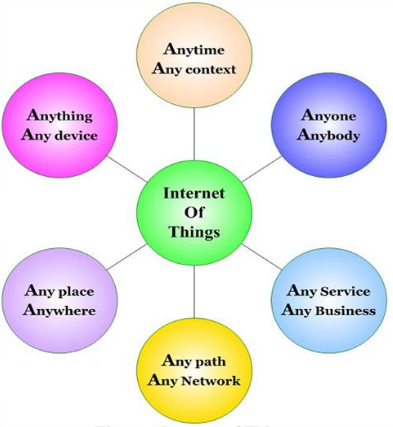
\includegraphics[0.55]{figures/IoT_definition.png}
            \caption{IoT kommunikation.\autocite{Sundmaeker2010}}\label{fig:IOTkom}
        \end{figure}
        Ved at overveje det nævnte kan IoT enheder defineres som enheder eller ting, som gennem trådløse forbindelser samt kabelforbindelser i et netværk er i stand til at samarbejde med andre forbundet enheder, se figur \ref{fig:IOTkom}. IoT enhederne er i stand til at skabe flydende kommunikation og kontekstuel service.\autocite{Hashmi2017}
        IoT enheder kan have følgende kommunikations mønstre: menneske til menneske, menneske til enhed, enhed til enhed.\\
        Dette vil altså sige at IoT enheder kan defineres som alt fra General Purpose Devices (Computere, printere, mobiltelefoner eller lign.) (GPD) til kaffemaskiner og toiletter tilkoblet wi-fi eller ethernet. Da GDP enheder er produceret af firmaer som Apple, hp, samsung og lenovo, er disse ofte produceret med kundernes sikkerhed i fokus. Rapporten har på baggrund af dette valgt at eksludere GPD enheder fra rapportens arbejdsområde, da disse ofte får software opdateringer der øger sikkerheden på produkterene.
        Arbejdsområdet indenfor IoT er altså reduceret til at være fokuseret på de produkter der kun nyligt er kommet på markedet, så som kaffemaskiner og toiletter med internet funktioner. \\


        \section{Valg af problem}
Herunder vil vi bedskrive hvilke problemer vi har valgt og hvorfor. 
    \subsection{Brainstorm}
    For at finde det problem vi vil arbejde med med henhold til Internet of Things, har vi lavet en brainstorm, der er opskrevet herunder.
        
        \begin{enumerate}
            \item Masser af hullede produkter på netværket.
            \item Et hul til at få adgang til alle IoT enheder. (Routeren)
            \item Nemmere botnet - Flere usikre enheder til at tilkoble et ondsindet botnet.
            \item Remote control - folk har nemmere ved ondsindet kontrol.
            \item Gammel software - Manglende software opdateringer til at lappe huller.
            \item Overvågning - Overvågning af enhederne, og deres brug.
            \item Datamining.
            \item Bliver mere kompliceret - Ældre mennesker kan have svære ved at bruge enhederne.
            \item Afhængig af IOT.
            \item Yderlige afhængig af mobil.
            \item Besparelse på varme og strøm.
            \item Jobovertagelse. 
            \item Flere faktorer kan give fejl på produktet.
        \end{enumerate}
    
    \subsection{Huller i netværket}
    Med firmaer som prioriterer indtjeningen over sikkerheden for deres klienter møder vi et marked som er fyldt med enheder som ikke har brugerens sikkerhed i mente og derfor udgør et sikkerhedsbrud for hele dit netværk. Dette åbner op for den mulighed at hackere kan tvinge sig adgang til dit netværk og bruge informationerne til ondsindede formål og på dette tidspunkt kan de IoT produkter som var skabt til at gøre din hverdag nemmere bruges imod dig. Dit smart TV kan tage billeder af dig, 
    
    \subsection{Remote control}
    IoT muliggøre at mange enheder som før skulle betjenes manuelt kan nu styres via fjernadgang. For forbrugeren kan dette være en stor fordel da flere opgaver kan udføres uden man fysiks skal bevæge sig. Sikkerhedsmæssigt kan det skabe problematikker da hvor der før kun var fysisk adgang til enheden er det nu muligt at tilgå enheden et vilkårligt sted fra netværket eller internettet. Ondsindetpersoner kan derfor overtage produktet og misbruge informationer eller udføre fysisk skade. Remote control kan være et problem men kun hvis der er huller i netværk sikkerheden og derfor vil det være bedre at fokusere på netværk sikkerheden.
    \subsection{Gammel software}
    Et af de store problemer vi så ved sikkerheden i IoT enheder var den relativt korte end of life tid på meget af softwaren og firmwaren involveret. Ved end of life vil en producent typisk stoppe med at lave nye opdateringer til deres produkt, og dette inkluderer sikkerhedsopdateringer. I følge eksperter er opdateret software er en af de absolut vigtigste ting %TODO: andet ord
    når det kommer til at være sikker online. \autocite{soups2015} Hvis software ikke bliver regelmæssigt opdateret vil den være langt mere sårbar, da den ikke vil være resistent mod de nyeste udviklinger inden for hackingangreb.
    \subsection{Problemanalyse}
    Hvad er jeres initierende undren?\\
    Da IoT bliver sådan en stor del af vores hverdag vil vi gerne kende de problemer der kan opstå.\\
    
    
    
    \subsection{HV spørgsmål}
    Hvorfor opstår dette problem?\\
    Fordi der bliver bygget IoT enheder som ikke har haft fokus på sikkerhed. Det sker da der er fordel i at komme først på markedet\\
    Hvorfor er det et relevant problem? \\
    Problemet bliver kun større. Det er et stadigt stigende antal devices.
    
    Hvad sker der hvis problemet ikke løses?\\
    Hvad er symptomerne? \\
    Hvad er effekten? \\
    
    
    Hvad?\\
    Hvilke begreber skal jeg være bekendt med for at kunne forstå dette problem?\\
    Hvordan begrebsliggøre andre dette problem?\\
    
    Hvem?\\
    Hvem er skyld i problemet?\\
    Hvem siger dette er et problem?\\
    Hvem påvirkes af dette prblem?\\
    Hvem har indflydelse på problemet?\\
    
    Hvor?\\
    Hvor opstår dette problem?\\
    Hvor har dette problem en effekt?\\
    
    Hvornår?\\
    Hvornår opstår dette problem?\\
    Hvornår begyndte dette problem først at opstå?\\
    
    \subsection{Problemtyper}
    Anomali\\
    Paradoks\\
    Beslutningsproblemer\\
    Normalier\\

        \section{Problemstilling}

IoT har som beskrevet et problem med at de bliver koblet på internettet hvor de så er udsatte for en lang række angreb fra ondsindet personer. Enhederne er i nogle tilfælde slet ikke egnet til at være på nettet da de ikke er udviklet med den nødvendige sikkerhed der skal til for at udgå at blive hacket. I sidste ende skaber usikre IoT enheder problemer for brugeren da andre enheder på netværket også kan blive påvirket af angrebet og enheden selv kan stoppe med at virke som den burde.\\

Hvad der skal skrives om:\\
* Hvad er problemet \\
* hvordan er det et problem\\
* \\
* \\
* \\


\section{Problemformulering}
%Hvordan kan den stadig stigende mængde af tilførte huller i netværk, lukkes uden at gennemføre lovgivninger.\\
Hvilke muligheder er der for at lukke forbindelsen mellem hackede enheder og personlige computere, uden at miste funktionalitet.
\\
%Hvilke sikkerheds risici eksistere i IoT enheder, som kan skabe huller i et lokalt netværk?
%Hvordan kan sikkerheds hullerne undgås?¨
\\

        %\section{Problemstilling}
Hvad der skal skrives om:
* Hvad er problemet 
* hvordan er det et problem
* 
*
*

        \printbibliography[heading=bibintoc]
        \label{bib:mybiblio}
        \printglossaries
        \listoftodos
    \end{spacing}
\end{document}